\documentclass[11pt,a4paper]{article}
\usepackage[hyperref]{naaclhlt2019}
\usepackage{times}
\usepackage{graphicx}
\graphicspath{ {./figs/} }
\usepackage{latexsym}
\usepackage{graphicx}
\usepackage{hyperref}
\usepackage{url}

\aclfinalcopy 

\title{Summarizing Political Discussion Forums}
   
\author{
  \begin{tabular}[t]{c@{\extracolsep{1em}}c}
    Shay Merchant   & {\tt merchants18@students.ecu.edu} \\ 
    Cason White     & {\tt whitecas18@students.ecu.edu} \\
    Dillon Roberts  & {\tt robertsd13@students.ecu.edu}\\
    Jacob Craiglow  & {\tt craiglowj16@students.ecu.edu}\\
  \end{tabular}
} 
\date{}
\begin{document}
\maketitle
\section{Introduction}
Often, bills submitted to Congress are long, involved, and confusing to understand.  This project aims to provide a simple, easy method of understanding these documents through mass summarization of bills that have been submitted through congress week by week, as well as a simple classification of these documents into a few  easy to understand categories. Our end goal is to allow the average user to look at some of the most recent bills that have been submitted, and quickly ascertain whether the bills is especially important, what the content is, and then, within a margin of error, what category the bill falls under, all within a short span of time. As far as the group members know, nothing similar to this has been created, though there are of course summarization tools that already exist, which makes creation of this tool especially exciting.  Congress.gov has provided a useful api, which has allowed the group members to grab documents by upload date, which has then enabled the summarization and classification of large numbers of documents without the creation of an involved scraper or web crawler.  The summarization itself was utilized using the gensim library, which implements a variation of LDA to process the documents in question.  Our classifier uses Naive-Bayes to classify documents into four separate categories, with a current accuracy rating of about 75\%, which is expected to climb higher as more documents are added to the classifier's corpus.  In general, the project is nearing it's conclusion, with the only real work left to be done is miscellaneous debugging and small quality of life improvements.

\section{Related work}
Milad Moradi’s group worked on a similar program.[2]
Rather than being focused on political documents, Moradi chose to focus on biomedical texts. Like us, Moradi outlines how the challenge they had to overcome was the different diseases and subcategories of biomedical texts which can affect the way a text is formatted. Moradi’s approach was to tackle summarization in 4 steps. Preprocessing, topic extraction, sentence clustering and summary generation. The pros of this approach is that it is concise and relatively simple to implement. The cons could be that a simple approach may take out some important language and context out of the original text to summarize it.  

Anna Kazantseva, and Stan Szpakowicz also had similar work with summarizing short stories.[3] Their team took a unique approach, whereas they made sure their reader knew certain details about the literature they were reading. The pro to this choice is that you are ensuring that your reader has some level of understanding at the end of the summary, even if the summary is less than ideal. The con to this approach is that a reader may have to have an understanding of the document before it’s summarizes, which could potentially contradict the point of a summary.  

The primary focus of NLP research in regards to legal texts has been within the field of paralegal work with a focus on "e-discovery", a  period within the confines of legislative action where the parties involved will gather evidence to support their arguments. The strongest forces within this research has came from the private sector as anyone posing any new advances has a strong financial stake to gain. In the field of politics the primary focus has been on bill success. This is a binary classification task where data is public ally available online which makes it well suited to solve with NLP techniques.

The most often used approach to the problem has been to utilize a machine learning with a neural network. Neural networks have the capacity to identify features about a text which are indicative of categories. Despite historical success of these language models there has been little success in identifying distinct and significant features about text which would indicate success or failure. Rather the most important features, as intuition might lead to, are contextual features such as the bill being supported by a senior committee member or being supported by the majority party.
In [9] Smith, Yano, and Wilkerson defined a baseline algorithm for measuring the likelihood of a bill being passed in the U.S Congress. Some 85\% of bills do not get passed, and nearly 90\% of bills that are recommended by a committee shall pass. The authors incorporated these findings with the application of linear regression based off of a bill's feature vectors.

In [9] Smith, Yano, and Wilkerson engineered a list of 11 basic measures which were centered around answering questions. These features specifically were found to be more telling than textual analysis for predicting a bill's classification into success or failure. Many of these measures had high prevalence across the set of data which does create some ambiguity in measuring their impact, as they noted.

In their approach [9]S, Y, and Wilkerson also applied 4 categories of bills to reduce prediction error. They differentiated bills into categories regarding trivial issues, technical changes to current laws, recurring issues, and important urgent issues such as the 9/11 terrorist attacks. Using this approach they were able label the data and utilized the 3 most commonly occurring categories of bills which were trivial, recurring, and important, to achieve an accuracy of of 83\% across prediction tasks. However, it was was found that this only produced a marginal improvement upon their baseline for prediction, but could act as a substitute in place of the originals.

The authors also viewed the data set in a bag-of-words representation with unigrams for text and bigrams for titles. With this they were able to create a model that outperformed predictions using a categorical model and a proxy vote model. They were able to deduce from this model that legislators often create bills with the expectation of their failure as a means of providing discussion for the issues that go along with them. Some bills also were found to have died for the fact that they were combined into larger, more encompassing bills.

The data itself has associated role call or voting information for which our experiment was unable to make use of. However, it is worth noting that the unigram and bigram views of data being able to discern features relating to any classification task were successful. The fact that the bag-of-words representation model surpassed that of the other models of the labeled data showed that the text itself held more data than most other features.

Nay[8] hypothesized that textual features about a data could be used to discern the probability of a bill's success. Their approach incorporated the word2vec algorithm. With this approach they were able to predict a probability of pass or failure with a high degree of accuracy. Ensemble learning methods were also applied in the form of random forests and GLMs. Along with this they also utilized a logistic regression to meta-learn from the outcome vector.

What was found of all the approaches proposed was that the combined power of word2vec with the ensemble learning created a a model with an AUC of 0.96 and MeanBrier score of 0.021, which showed the model's success. As with the previous experiments with the task and data it was found that the sponsor being of the majority political party was a key feature in determining success of a bill. With the success of the model it can be shown that the data is well suited to categorization tasks. As with the previous approach however the data is only labeled in this particular regard, not in a topical sense.

\section{Your approach}
As stated earlier, we are striving to make legislation more approachable. We have decided that the best way is to directly view the legislation itself. Politicians employ rhetoric and lie however, this is the word of the law. The words these documents contain will come to directly affect every citizen in the country. It is best toview them directly. However, they are almost deliberately padded and fluffed. Hidden behind a wall of jargon. This is an obvious job for NLP tools. There are a few different parts to project that we will discuss here. First we will detail the tools we use to accomplish this. 

\subsection{Tools}
Most code has been handwritten. The only heavy lifting library we have used is \href{https://radimrehurek.com/gensim/}{Gensim}. Gensim is a robust NLP open source library containing many different tools from stopword removal to Topic Modeling. We use it's stopwords list as a basis as well as its \href{https://radimrehurek.com/gensim/summarization/summariser.html}{TextRank summarizer}. We decided to use this as its implementation of TextRank is well tuned to our needs and we'd be hard pressed to improve upon it. 

The only other tool of note is Python's local JSON library. Our documents come in a json object from the API and thus this simplified the extraction process. 

Everything else you see in this project was hand coded to fit our needs.

\subsection{Data Gathering}
First we decided it would be best to be able to gather documents within the application. Somewhat fortunately, within the last couple years the US Government has implemented a useful API. This allows us to gather our data inclusively. 
To do this we will capture bills matching date criteria from an API at https://api.govinfo.gov/collections/BILLS/. The API is maintained by the government and contains valuable information about the logistics of each political document as well as the document itself. We are able to give a specific span of time to the API and receive all political documents that it has access to. These come in the for of JSON objects with metadata pertaining to each document. If you were to call this API on an older document, you would notice that you would not be able to. This API was created fairly recently. And lots of documents were added at one time. So while you are able to get documents from years back, you will want to pay special attention to the “dateIssued” value of the received JSON file. This value will give you the proper date of the bill. 

\subsection{Tokenization}
As with most of NLP, a mantra to keep in mind is “Garbage in, Garbage out.” So we took care to clean our documents. One interesting aspect of govinfo legal documents is the different stop words that must be taken into account for good classification and summarization. The documents are not very clean and contain many programmatic artifacts such as “[document]”, “head”, “script”, etc. These can cause serious misclassifications and must be removed in preprocessing. We also remove traditional stopwords such as “and”, ”of”, ”the”, etc. After this we construct a bag of words representation of each individual document to feed to our classifier. 

\subsection{Classification}
After stopword removal and tokenizing the data, it is classified by Naïve Bayes into one of four categories. Firearms/Explosive, Government/Political, Environment/Weather, Healthcare/Medicine/Welfare bill. These four categories were chosen as together they cover a broad spectrum of the political sphere. Firearms pertain to legislation regarding firearm and ammunition usage. As well as  purchasing rights. The political label is a nebulous one that consists of legislation affecting the state of our legislate, judicial, and executive branches. This includes everything from salary adjustments to procurement of naval vessels in international waters. The Environmental label consists of legislation dealing with pollution standards and wildlife. This can also include things like national park budgeting and other forms of preservation. Finally, the medical label Simply deals with anything regarding prescriptions, to drug trade, medicare, or insurance. It is another very nebulous topic however, extremely important in our current political climate. To train our model, eighty bills and joint resolutions occurring in the past year were hand annotated and classified into one of these four categories. As a proof of concept we found twenty training docs for each classification. Bills can vary wildly in length so special care was taken to curate bills of similar lengths for each category. Initial failure to do so resulted in false classifications. After training we can feed our classifier new documents.We also made sure each bill was very recent. This is important as topics and language can change wildly as time progresses and congress members rotate out. After cleaning and tokenizating our documents they are sent to the classifer. Our classifier trains on initialization due to the small amount of training data. However this is easily saved and loaded once the project scales. Upon call we compute the log posterior of the document and labels and return the most probable classification. 

Our classifier was then tested and found to have an accuracy of 75\% (see 6.1). Our test data consisted of bills gathered from a similar time and were also hand annotated. We surmise that this accuracy is simply a lack of training data. As all our documents are bills, much of the language is political jargon and very similar from document to document. With more data our classifier will be able to properly weight the distinguishing terms. Given our small training data set we thought four classifications should suffice as proof Naïve Bayes is feasible for the purpose of bill classification.

\subsection{Summaraization}
Following classification we then create a multi-sentence summary of the documents. This is accomplished by Gensim’s summarize function. Gensim uses the TextRank algorithm initially presented by Rada Mihalcea and Paul Tarau of the University of North Texas. Textrank is a graph-based ranking algorithm that sets sentences as nodes on a graph. It takes the degree of each node as a rank with the highest ranking sentences being most important. This is determined by similarity to other sentences. Essentially, the sentence most similar to the most sentences in the document is considered the most important sentence. Then the summary is based off the connected vertices. 

Gensim's summarize takes two parameters. The document and a ratio. We set a ratio of 0.75. This ratio essentially controls the proportion of summary sentences to document sentences. A proportion of three-fourths gives us a solid summary while still cutting potentially unnecessary information. This preserves our initial mission statement. Due to the nature of gensim’s TextRank summarization algorithm there is no need to train any models as it is unsupervised. Much of the work lies in proper preprocessing of the data and tuning of the pre-existing algorithm in order to best suit the document. We then display the bill metadata, classification, and the summary. 

\subsection{Milestones \& Schedule}

Our original schedule was vastly different from what actually occurred. We created the preprocessing code on schedule. However, when attempting to build the LDA modeler we had a major direction shift. Originally we were going to build topic models and a summarizer for daily congressional transcripts. However, we then decided it would be more useful to go directly to the legislation and summarize this instead. This meant dropping topic modeling as these documents were much shorter. This came together quickly over the course of two weeks. Then another week for rigorous testing. In the past few weeks we then decided this could benefit from document classification. So we implemented the Naive Bayes classifier discussed previously. All that is left to do is construct a larger set of training data in order to tune the classifier and possibly implement a way of saving the model to the disk and loading one up. Following this, our energy will be spent preparing and recording our presentation. 

\subsection{Git Links and Directory Discussion}
Here we will break down our git methodology and project structure. 

We opted for the basic git workflow with a single branch and communicating our changes in our tri-weekly meetings. Our directory structure is similarly simple. All of our code is located in the src/classifier folder. This contains the Naive Bayes, user interface, API, and summarizer code. Currently it also contains our training and test data. However, this will be moved to our data folder promptly. The pub folder contains all textual project information including the readme.md as well as our previous progress reports and initial proposal. 

\begin{enumerate}
    \item \href{https://gitlab.com/Merchant89/b/-/blob/master/src/Classifer/UserInterface.py}{User Interface} - Driving code. Gives the user the option of viewing bills or joint resolutions. It then asks the user what date range they would like to view. As well as a shortcut to the past weeks.
    \item \href{https://gitlab.com/Merchant89/b/-/blob/master/src/Classifer/WebsiteInfoGetter.py}{API} - WebsiteInfoGetter is built to query the https://api.govinfo.gov/collections/BILLS/ API for a user specified set of bills. The user will ask for a specific range of dates. 
    \item \href{https://gitlab.com/Merchant89/b/-/blob/master/src/Classifer/ResolutionSummarizer.py}{Summarizer} - This contains the code built to summarize either a bill or a joint resolution. This also runs the Classifier on the document. 
    \item \href{https://gitlab.com/Merchant89/b/-/blob/master/src/Classifer/NaiveClassifier.py}{Naive Bayes Classifier} - This is the file containing all of the Naive Bayes code including training, testing, and querying.
    \item \href{https://gitlab.com/Merchant89/b/-/tree/master/src/Classifer/train}{Training Data} - Currently in src/classifier folder but will be moved to data presently.
    
\end{enumerate}
\section{Data}

When choosing our data set, we made sure that our data would be readily accessible and plentiful. A personal requirement for the data set, was our data had to be something that is relatable, something interesting, and something that could matter to a lot of people. The data that this will run on will be transcripts from congressional-record the United States Congress.[4] \\
The LDA algorithm is an unsupervised learning algorithm and thus does not require a training set persay. However, there will be testing done on small increments of a day's transcript throughout the length of the project. This data is freely available for download from congress.gov and is the main focus of our work. Its contents are records of politicians discussing issues stored in PDF format. This can be parsed using pdfminer, a Python library.

The progress in our dataset is that our group is using data compiled from congressional records.[4] The congressional records have been recorded, and are accessible for every week day since 1994. This gives us roughly 6,760 documents to access. Each of these documents range in size depending on the amount discussed or the amount done in congress that day. On average each document is around 150-300 pages in length. This larger document is also available in many separate, smaller sub-categorical text documents. The sub-categories are daily digest, extension of remarks, House and Senate. The daily digest provides an extremely brief and undescriptive synopsis of the events that occured that day. The extension of remarks is just an extension to remarks on the senate floor given to the recorder after the event has occured. Lastly, the House and Senate contain our main focus and contain the data of all the events that occured that day in detail. 

Our original intent for these documents was for our program to be able to access any one of these documents and summarize it. Once it became clear this was beyond the scope of our planned summarizer, we narrowed our focus on specific portions of the original full documents. We decided to focus on specific sub documents we deemed important. This allowed our summarizer to perform a much better job at summarizing the text. Because these documents were also available as text, it also allowed us to disregard the use of pdfminer, and use the text documents directly. Lastly, we will be experimenting with summarizing the specific subsection of Public Bills And Resolutions and Private Bills and Resolutions. These seem like the most viable source to summarize as they are split by the header "H.R" followed by the bill's resolution number. This would viable in the sense, we can split each of the bill's and resolutions easily, summarize them, and present them to the user. 

Once we accomplish the summarizing of Bill Resolution's, we may use the larger data set to experiment with other forms of summarizing, such as keyword summarizing or summarizing larger bodies of political text with visualizations.  


\section{Tools}
We will be using various tools to execute our program. Below is an outline of the tools we intend to utilize and what they will be responsible for.
\subsection{Corpus Retrieval}
We intend to utilize Python libraries to retrieve pdfs on demand from the live website: \url{Congress.Gov}. We specifically beleive that either the library "wget" or "requests" shall be appropriate for our needs. We believe, given additional opporunity for development, that we could utilize a database where the processed plain text portion of the pdfs could be stored.
\subsection{Preprocessing}
There are many libraries for assisting with preprocessing in the Python language. To strip the text out of pdf format we intend to utilize the "pdfminer" library, which also offers additional features which we believe will prove useful for understanding the structure of the corpus. Specifically, we intend to utilize the ability of pdfminer to recognize sections of pdf documents and extract headers in a way that we might leverage in our model.\\
After pdfminer has extracted our corpus, we intend to perform remainder of our preprocessing with the Python library "nltk". Nltk supports tokenization, stemming, lemmatization, among other useful preprocessing features.
\subsection{Summarization Application}
Preprocessing for TextRank is simple and nearly finished. We extract the bill summary from its place in the document. Then the algorithm converts it to lowercase and removes some general stopwords. This incorporates one document of our corpus. This works fine however we are still nailing down the proper stopwords to remove as legal jargon is much different from conversational speech. \newline
\newline
Currently all tuning is done manually and not on the fly resulting in less than ideal summaries for nearly all our input data. The ideal summary for a document is one to two extracted succinct sentences. Because the algorithm is usually not tuned to fit a specific document, several more sentences than necessary is produced. These tend to be garbled and nonsensical or no summary at all for very small docs. TextRank uses a ratio representing the number of sentences in a document to the number of sentences in the produced summary. The tuning will be based on the number of sentences present in the document. 

 \subsection{Data Visualization}
  We believe that data visualization is an integral piece to understanding the output of something as complex as topic modeling. Thus, we intend to utilize "matplotlib", a Python library to tabulate our results. We also hope that we may be able to integrate the library "pyLDAvis" to create more visually interesting results.\\
  If given enough time, we also hope to present our project as a usable application where a user may keep track of select topics that they may receive alerts on when they come up in the Congressional conversation. We believe that this would be a very useful tool for a reports on these conversations which are not often discussed or reported with minimal bias in modern American news media.\\
  The current focus of our data as stated in previous sections is on the bills of the House and Senate. These documents are stored in XML format, and since 2013 have been maintained online in an easily accessible form. As XML is a formatted language it is trivial to obtain specific elements of these documents. We believe that one measure that might be important to human interpretation of the quality of our summarizer.\\
  
  One interesting visualization we believe could be integrated is some kind of visualizer that could relate a "profile" with what keywords they tended to vote for or against. This could be integrated into an application that could be queried for something such as "what bills did senator John Doe vote for which they statistically don't?", or "what did the Congress members who voted on this bill have most in common". 
  
  There exists additional data to support this kind of feature on the site and we believe that visualizations such as those mentioned would be very useful in contributing to the community of knowledge for informing American voters, and maybe nations around the world if our approach was duplicated.\\
  While the data was presented in an XML format it was very "dirty", being difficult to discriminate between formatting data and language we intended to target. We believe this will be one of the biggest challenges of analyzing the corpora with NLP. 
  
  The results of our attempts were not in vain, however, as we were able to apply Gensim's keyword function to create a bag of words representation of keyword-document frequencies. The tokens which occurred the most as keywords in a set of testing data that consisted of 122 documents showed that the raw data from navigating elements in the XML tree were "dirty", so we ignored the first 14 of them in the infographic and found more meaningful keyword frequencies. We chose to use a small fraction of the corpus as navigating XML trees proves computationally expensive along with keyword generation.\\
  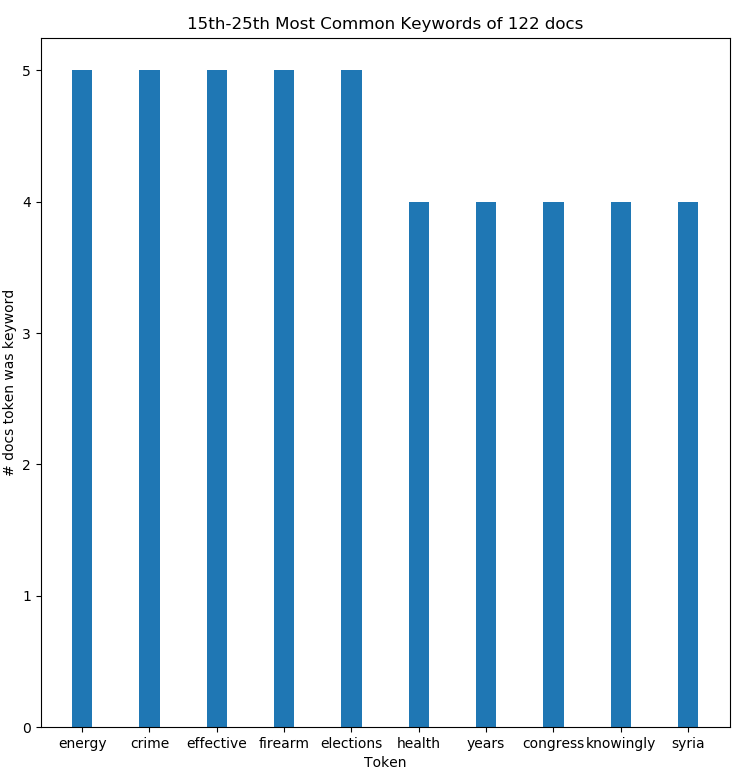
\includegraphics[scale=0.5]{test_kw-mostcommon_15-25}
  
  This graph represents the most common keywords of 122 documents. From this data we decided to to seperate Bill's into 4 main Bill labels. The labels are environment, health, firearms, and government. Below is an example of the results of the most common keywords being seperated by label. As seen, some words are ambiguous and can be shared by more than one label.  
  
 
 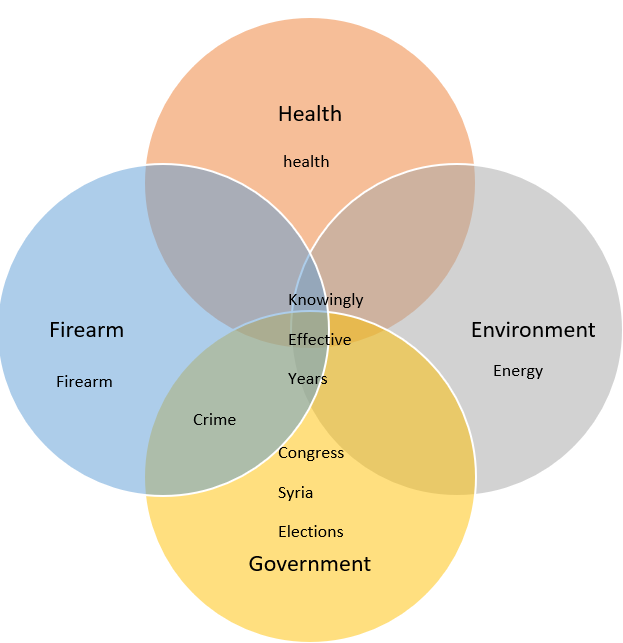
\includegraphics[scale=.60]{figs/Venn.PNG}
 
  
  \section{Data and Results}
  Taking our health, firearm, government, and environment labels we set up a classifier using Naive Bayes. This Naive Bayes classifier was then trained with 20, full length Bill's for each label. The training data produced the following top ten keywords for each label. This can be reproduced by running our NaiveClassifier script with the built in function top\_n.
  \newline\newline
  \noindent
  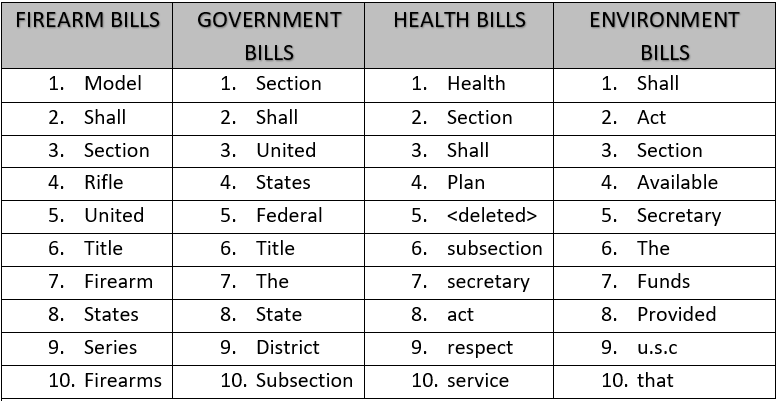
\includegraphics[scale=.60]{figs/naivetop.PNG}
  \newline\newline
  \noindent
  Running our Naive Bayes classifier on a random selection of Bill's from our 4 catagories, firearm, government, health and environment we were able to achieve an accuracy of 75 percent. This accuracy was calculated by using a simple formula of 
  \[ Label Accuracy = \frac {Labels Correct}{Total Labels} * 100\]
  This can be reproduced using our NaiveClassifier script with the function evaluate\_classifier\_accuracy.This accuracy is also displayed when running our program normally from the UserInterface script.
  Our original goal was to decipher Government Bill's. Here is a success and a failure of our classifier on a couple interesting Bills.
 
 
 \noindent\textbf{Successful summary:}

 \noindent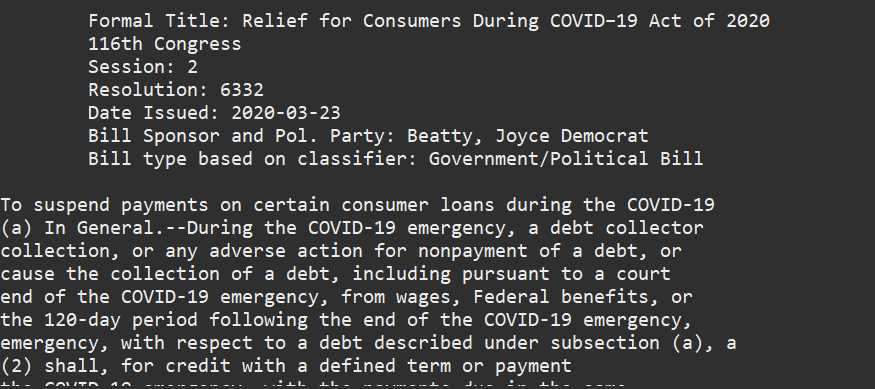
\includegraphics[scale=.60]{figs/Screenshot2.PNG}
 \newlinenewline\noindent\textbf{Unsuccessful summary:}
  \newline
  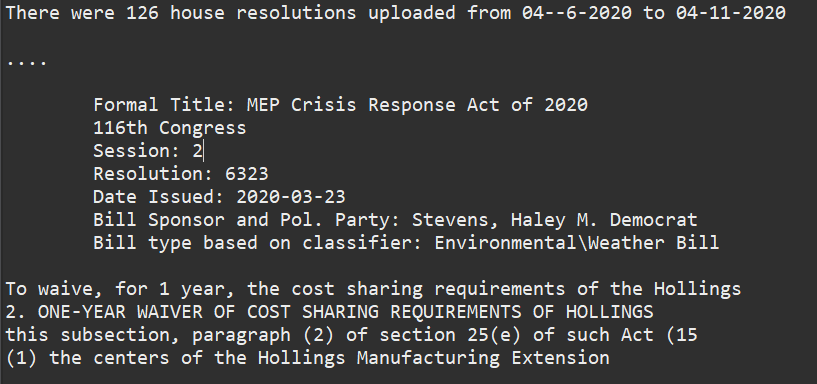
\includegraphics[scale=.60]{figs/Screenshot3.PNG}
  \newline
  
    In the first summary, the classifier is able to classify this Bill as a political Bill, despite the deceptive content of COVID-19 and implications of it being a health bill. The Bill is actually about debt and federal benefits.
  The second Bill is successfully summarized but unsuccessfully classified. The Bill has been classified as a environmental Bill, while the Bill is about giving manufacturing employees the "resources" and ability to work during the COVID crisis. This misclassification is an issue we faced on Bill's that shared many common words with other Bill's. In this case, the Bill referenced resources, which is commonly found in environmental Bills. Both of these examples can be found running our UserInterface script. These two particular Bill's were summarized from the "House Resolutions from this Week" option.

  
  
\section{Conclusion and future work}
The data has historically shown to be applicable to the task of classification. We set forth upon the task of summarization and achieved success utilizing LDA. Specifically, it has been shown that even with a rudimentary model viewing only 4 topics that some bills can be discovered to be part of certain topics despite what the title of a bill may lead the reader to believe. This realization should be taken into account in future works as previously title's were seen as significant features which should be viewed differently - not features that could hide an agenda. With future work there should also be some integration of unsupervised machine learning techniques given the proven success that they have to the task of summarization such that topics can be discovered and aggregated for the data set.
  
  

\clearpage
\section{References}

[1] Los Angeles Times. (2011, June 19). Congress turns bill titles into acts of exaggeration. Retrieved from https://www.latimes.com/world/la-xpm-2011-jun-19-la-na-0620-titles-20110620-story.html 
\newline
\newline
[2] Moradi, M. (2018, November 13). CIBS: A biomedical text summarizer using topic-based sentence clustering. Retrieved from https://www.sciencedirect.com/science/article/pii/S1532046418302156?via=ihub 
\newline
\newline
[3]Kazantseva, A. (n.d.). Summarizing Short Stories. Retrieved from https://www.aclweb.org/anthology/J10-1003.pdf 
\newline
\newline
[4] (n.d.). Retrieved from https://www.govinfo.gov/app/collection/crec/2020/01/01-10/6/{"pageSize":"20","offset":"0"} 
\newline
\newline
[5] Gensim Link:
https://radimrehurek.com/gensim/
\newline
\newline
[6] Gensim Summarizer:
https://radimrehurek.com/gensim/summarization/summariser.html
\newline
\newline
[7] Mihalcea, R., & Tarau, P. (2004, July). Textrank: Bringing order into text. In Proceedings of the 2004 conference on empirical methods in natural language processing (pp. 404-411).
https://web.eecs.umich.edu/~mihalcea/papers/mihalcea.emnlp04.pdf \end{document}
\newline
\newline
[8]Nay J. J. (2017). Predicting and understanding law-making with word vectors and an ensemble model. PloS one, 12(5), e0176999. https://doi.org/10.1371/journal.pone.0176999
\newline
\newline
[9] Yano, T., Smith, N. A., & Wilkerson, J. D. (2012, June). Textual predictors of bill survival in congressional committees. In Proceedings of the 2012 Conference of the North American Chapter of the Association for Computational Linguistics: Human Language Technologies (pp. 793-802). Association for Computational Linguistics.